% !TeX root = RJwrapper.tex
\title{An overview of R packages for single-source capture-recapture
models}
\author{by Maciej Beręsewicz and Piotr Chlebicki}

\maketitle

\abstract{%
In this paper we provide an overview of R packages that allow to fit
various single-source capture-recapture (SSCR) models. In genera, SSCR
approaches assume that capture history follows certain distribution
(e.g.~negative binomial, poisson, one-inflated poisson) but the
observational data consist only positive counts i.e.~we observe zero
truncated distributions.
}

\hypertarget{introduction}{%
\subsection{Introduction}\label{introduction}}

Introductory section which may include references in parentheses
\citep{R}, or cite a reference such as \citet{R} in the text.

\hypertarget{single-source-capture-recapture-models}{%
\subsection{Single-source capture-recapture
models}\label{single-source-capture-recapture-models}}

\citet{Bohning2022}

\hypertarget{r-package-for-single-source-capture-recapture-model}{%
\subsection{R package for single-source capture-recapture
model}\label{r-package-for-single-source-capture-recapture-model}}

This section may contain a figure such as Figure \ref{fig:Rlogo}.

\begin{Schunk}
\begin{figure}[htbp]

{\centering 
\includegraphics[width=2in]{Rlogo} 

}

\caption[The logo of R]{The logo of R.}\label{fig:Rlogo}
\end{figure}
\end{Schunk}

\hypertarget{truncated-discrete-distributions}{%
\subsubsection{Truncated discrete
distributions}\label{truncated-discrete-distributions}}

In order to use truncated distributions we may use default functions
truncaed at 0

\hypertarget{countreg}{%
\subsubsection{countreg}\label{countreg}}

\texttt{countreg} package includes function \texttt{zerotrunc}

\hypertarget{vgam}{%
\subsubsection{VGAM}\label{vgam}}

The most advanced

\hypertarget{stan-and-brms}{%
\subsubsection{stan and brms}\label{stan-and-brms}}

\hypertarget{case-studies}{%
\subsection{Case studies}\label{case-studies}}

There will likely be several sections, perhaps including code snippets,
such as:

\begin{Schunk}
\begin{Sinput}
x <- 1:10
plot(x)
\end{Sinput}

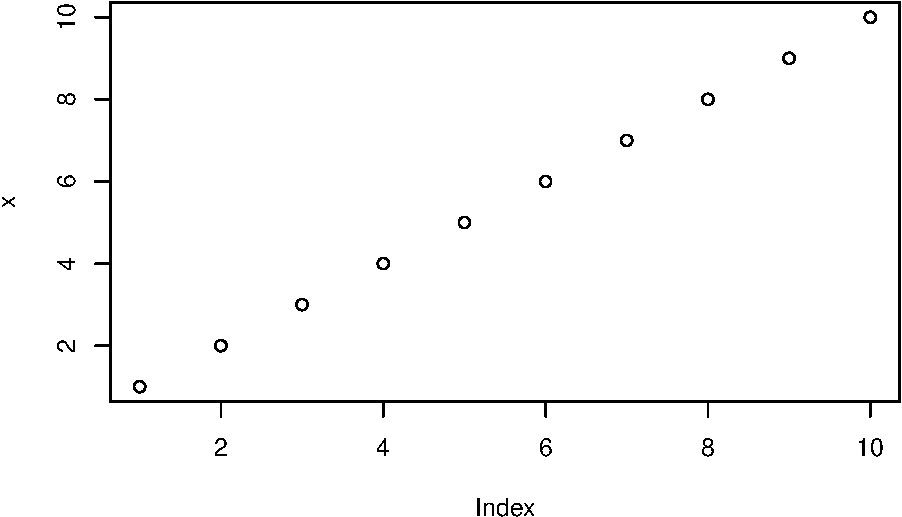
\includegraphics{overview-single-source_files/figure-latex/unnamed-chunk-1-1} \end{Schunk}

\hypertarget{summary}{%
\subsection{Summary}\label{summary}}

This file is only a basic article template. For full details of
\emph{The R Journal} style and information on how to prepare your
article for submission, see the
\href{https://journal.r-project.org/share/author-guide.pdf}{Instructions
for Authors}.

\bibliography{overview-single-source.bib}

\address{%
Maciej Beręsewicz\\
Poznań University of Economics and Business\\%
Al. Niepodległości 10\\ 61-875 Poznań, Poland\\
Statistical Office in Poznań\\%
ul. Wojska Polskiego 27/29\\ 60-624 Poznań, Poland\\
%
\url{https://ncn-foreigners.github.io/}\\%
\textit{ORCiD: \href{https://orcid.org/0000-0002-8281-4301}{0000-0002-8281-4301}}\\%
\href{mailto:maciej.beresewicz@ue.poznan.pl}{\nolinkurl{maciej.beresewicz@ue.poznan.pl}}%
}

\address{%
Piotr Chlebicki\\
Adam Mickiewicz University\\%
ul. Wieniawskiego 1\\ 61-712 Poznań, Poland\\
%
\url{https://github.com/Kertoo}\\%
%
\href{mailto:piochl@st.amu.edu.pl}{\nolinkurl{piochl@st.amu.edu.pl}}%
}
